\label{sec:data}
% Main characteristics of the data set: source, type of data
% Description of variables used for the	analysis and correspondence with the (ideal) magnitudes in the empirical specification
% Descriptive statistics of the	main variables in the analysis

Data on airports and connections is available at: \href{https://openflights.org/data.html}{openflights.org/data.html}. See Figure \ref{fig:airports} below. The dataset includes an airport identifier (IATA code), location data (latitude and longitude), and various characteristics of the airport (country, city, altitude etc.).
Furthermore, the dataset contains connections between airports (67,663 routes between 3,321 airports on 548 airlines). %Airports are identified using the IATA code.%we already mentioned this above
\medskip\\
Data on prices are scraped from the internet. Various sites contain flight prices (Skyscanner, Momondo, Flightfinder, Expedia mv.). Our choice of site will be guided by practical concerns.
\par
Alternative data:  \url{http://stat-computing.org/dataexpo/2009/}
\begin{figure}[H]
  \centering
  \caption{Airports}
    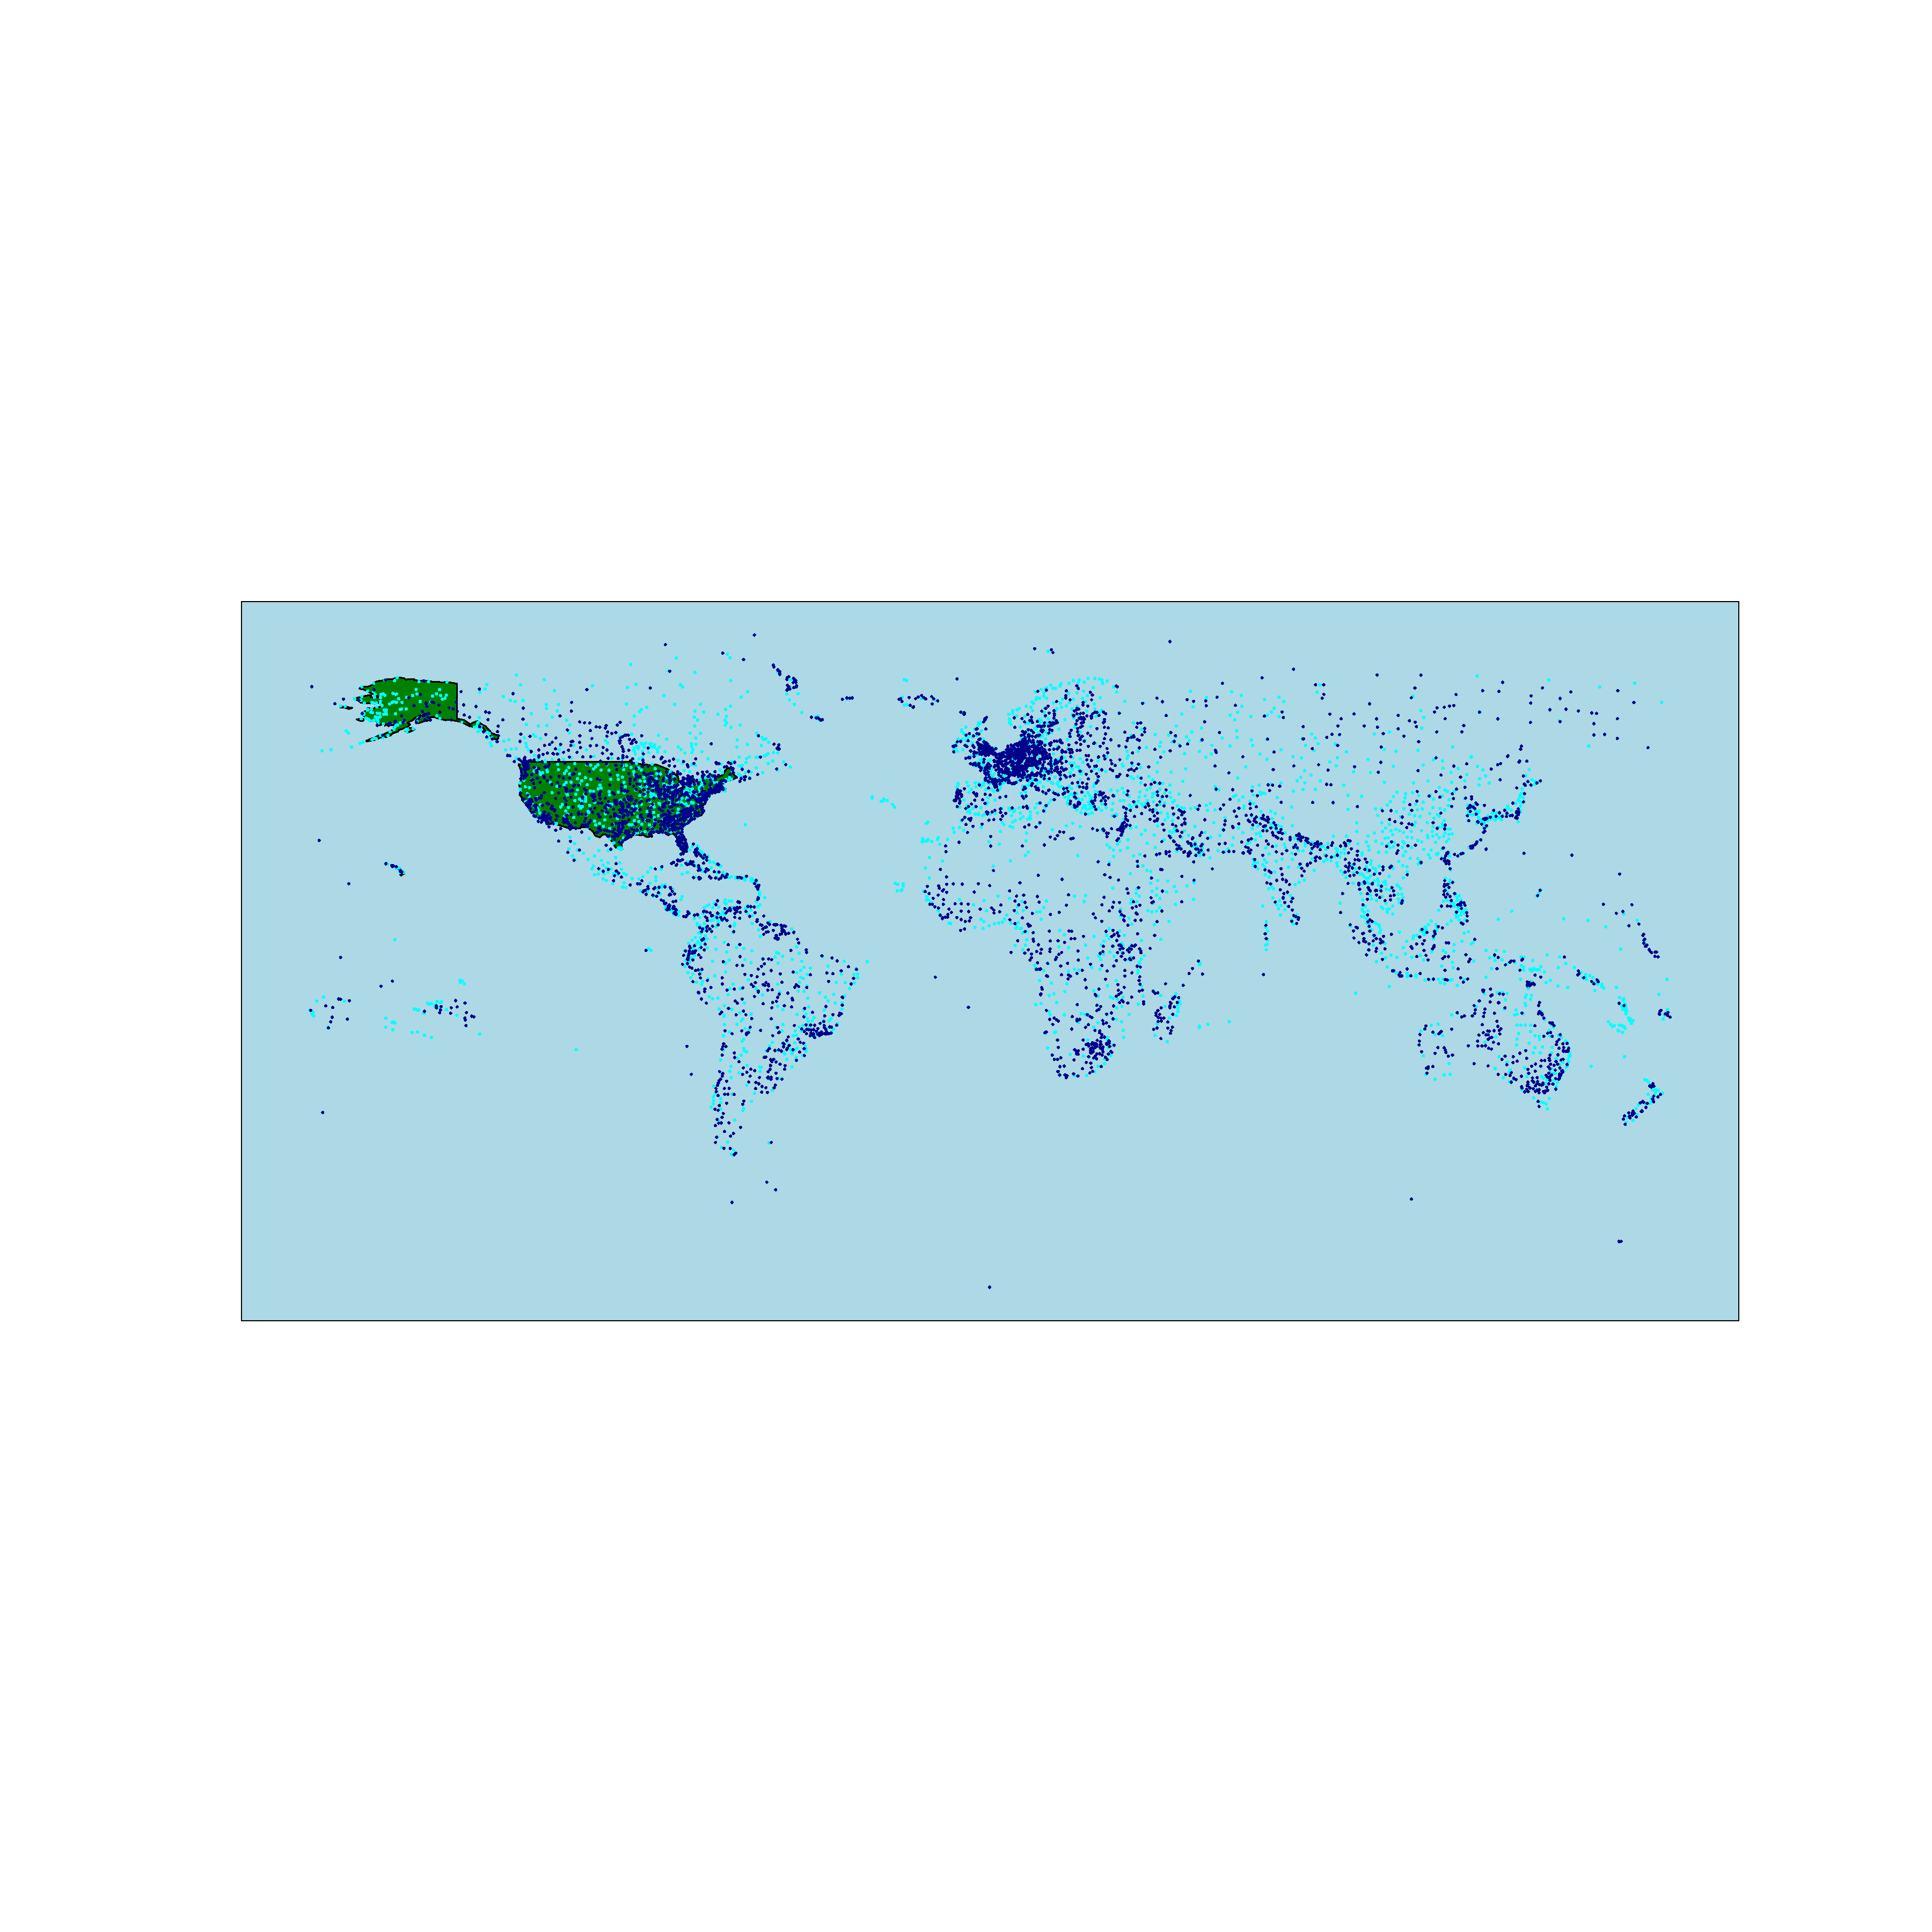
\includegraphics[width=1. \textwidth]{Exam/Airports_WorldMap}
  \label{fig:airports}
\end{figure}
